\documentclass[10pt]{beamer}  % pour la présentation
%\documentclass[10pt,handout]{beamer}  % pour les notes de cours


\usetheme{Antibes}
\usecolortheme{whale}
\setbeamertemplate{navigation symbols}{}
\setbeamertemplate{mini frames}{} % Supprime les petits cercles dans le header
\setbeamertemplate{items}[triangle]
\setbeamercolor{itemize item}{fg=black}
\setbeamercolor{itemize subitem}{fg=gray}
\setbeamertemplate{frametitle continuation}{}


\usepackage[utf8]{inputenc}
\usepackage[T1]{fontenc}
\usepackage[french]{babel}
\usepackage{amsmath, amssymb}
\usepackage{hyperref}
\usepackage{graphicx}
\usepackage{caption}
\usepackage{tikz}
\usetikzlibrary{shapes.geometric, positioning}
\usepackage{nicematrix}

%\newcommand{\Var}[1]{\mathbb{V}\mathrm{ar}\left[ #1 \right]}
%\newcommand{\Cov}[1]{\mathbb{C}\mathrm{ov}\left[ #1 \right]}
\newcommand{\E}[1]{\operatorname{\mathbb{E}}\left[#1\right]}
\newcommand{\Var}[1]{\operatorname{\mathbb{V}ar}\left[#1\right]}
\newcommand{\Cov}[1]{\operatorname{\mathbb{C}ov}\left[#1\right]}
\newcommand{\sigeps}{\sigma_{\epsilon}^2}
\newcommand{\ET}[1][]{\operatorname{ET}\ifx&#1&\else\left[#1\right]\fi}
\newcommand{\diag}{\operatorname{diag}}
\newcommand{\cote}{\operatorname{cote}}
\newcommand{\score}[1]{\operatorname{score}\left(#1\right)}
\newcommand{\logit}[1]{\operatorname{logit}\left(#1\right)}

\title{Apprentissage Automatique - L3 - KMAXPP05}
\subtitle{Chapitre 2 : Régions de prédiction et intervalles de confiance}
\author{Cédric Campguilhem}
\institute[]{
	Airbus Operations \\
	\href{mailto:cedric.campguilhem@airbus.com}{\texttt{cedric.campguilhem@airbus.com}}
}
\date{2025-2026}

\begin{document}
	
\begin{frame}
	\titlepage
\end{frame}
	
%=======================================================================================

\section[Introduction]{Introduction}

\begin{frame}{Problématique}
	\begin{itemize}
		\item Jusqu'à présent nous avons vu comment les modèles peuvent faire une prédiction pour des entrées $X$. Et globalement comment les modèles se comportent grâce à différentes métriques. Ou même comment localement on peut décomposer l'erreur sur des données de test. 
		\pause
		\item Mais pour une prédiction du modèle, dont nous ne connaissons pas le résultat vrai, quelle est l'erreur commise ?
		\pause
		\item Dans tous les domaines d'application, une erreur de prédiction a un \textbf{coût}.
	\end{itemize}
\end{frame}

\begin{frame}{Problématique}
	\begin{block}{Problématique}
		Tous les modèles sont des approximations. Essentiellement, tous les modèles sont faux, mais certains sont utiles. Cependant, il ne faut jamais perdre de vue le caractère approximatif du modèle. \\
		\vspace{0.5cm}
		\hfill
		\textit{--- Georges E. P. Box (2007)}
	\end{block}
	\vfill 
	\tiny \textcolor{gray}{Source: Response Surfaces, Mixtures, and Ridge Analyses - George E. P. Box, Norman R. Draper  - 2007 - p.414, John Wiley \& Sons}
\end{frame}

\begin{frame}{Régions de prédiction et intervalles de confiance}
	Dans ce cours nous introduirons les notions de régions de prédiction et d'intervalles de confiance, à la fois pour des problèmes de classification et pour des problèmes de régression.
	\begin{itemize}
		\item Dans un premier temps on développera l'intuition sur ces intervalles avant d'en donner une définition.
		\pause
		\item Ensuite nous verrons que les modèles linéaires (régression et classification) proposent des estimations théoriques de ces régions et intervalles.
		\pause
		\item Enfin, nous verrons comment, empiriquement, on peut établir ces régions et intervalles pour une grande variété de modèles.
	\end{itemize}
\end{frame}

%=======================================================================================

\section[Intuition et définitions]{Intuition et définitions}

\subsection[Intuition]{Intuition}

\begin{frame}{Présentation du cas d'étude}
	Nous considérerons le cas d'étude suivant:
	\begin{itemize}
		\item Supposons que nous voulions connaitre la taille moyenne des individus sur le campus de l'Université de Toulouse 3.
		\pause
		\item Il existe une valeur \textbf{vraie}. C'est la valeur que l'on obtiendrait si on mesurait \textit{tout le monde}.
		\pause
		\item En pratique, on travaillera avec des \textbf{échantillons}.
	\end{itemize}
\end{frame}

\begin{frame}{Construction des intervalles}
	Pour l'intervalle de prédiction:
	\begin{itemize}
		\item On collecte les tailles de $n$ étudiant(e)s.
		\item On cherche un estimateur de maximum de vraisemblance pour les \textbf{tailles} avec une distribution Gaussienne.
		\item On calcule l'intervalle centré représentant 95\% des \textbf{tailles} mesurées.
	\end{itemize}
	\pause
	Pour l'intervalle de confiance:
	\begin{itemize}
		\item On génère $m$ échantillons:
			\begin{itemize}
				\item On collecte les tailles de $n$ étudiant(e)s.
				\item On calcule la taille moyenne de l'échantillon.
			\end{itemize}		
		\item On cherche un estimateur de maximum de vraisemblance pour les \textbf{moyennes} avec une distribution Gaussienne.
		\item On calcule l'intervalle centré représentant 95\% des \textbf{moyennes} mesurées.
	\end{itemize}
\end{frame}
	
\begin{frame}{Résultats avec $n = 30$ et $m = 100$}
	\begin{columns}
		\begin{column}{0.5\textwidth}
			\begin{figure}
				\centering
				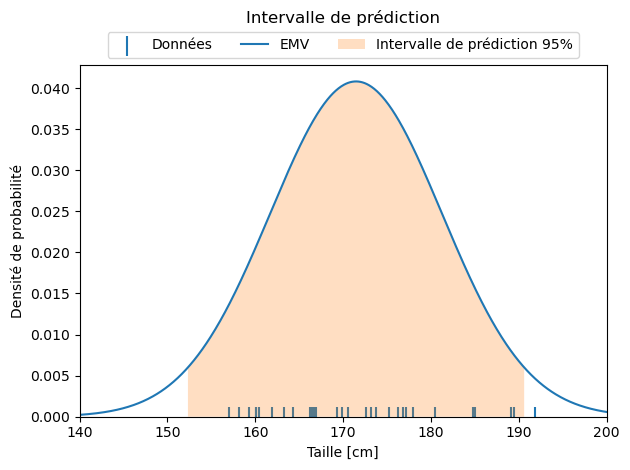
\includegraphics[width=1.0\linewidth]{Images/intervalle_prediction_n30}
				\label{fig:intervalle-prediction-n30}
			\end{figure}
		\end{column}
		\begin{column}{0.5\textwidth}
			\begin{figure}
				\centering
				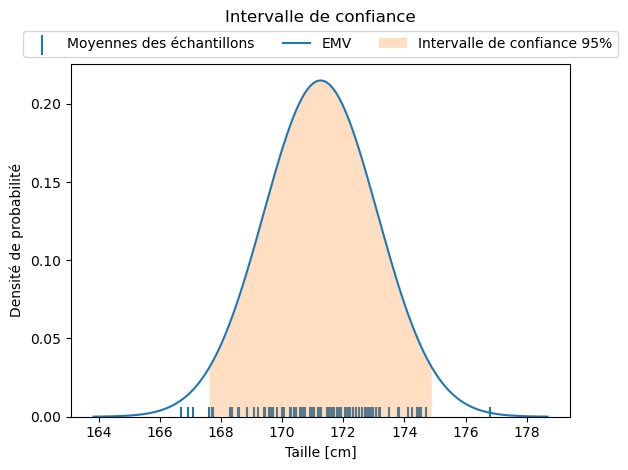
\includegraphics[width=1.0\linewidth]{Images/intervalle_confiance_n30}
				\label{fig:intervalle-confiance-n30}
			\end{figure}
		\end{column}
	\end{columns}
\end{frame}

\begin{frame}{Résultats avec $n = 300$ et $m = 100$}
	\begin{columns}
		\begin{column}{0.5\textwidth}
			\begin{figure}
				\centering
				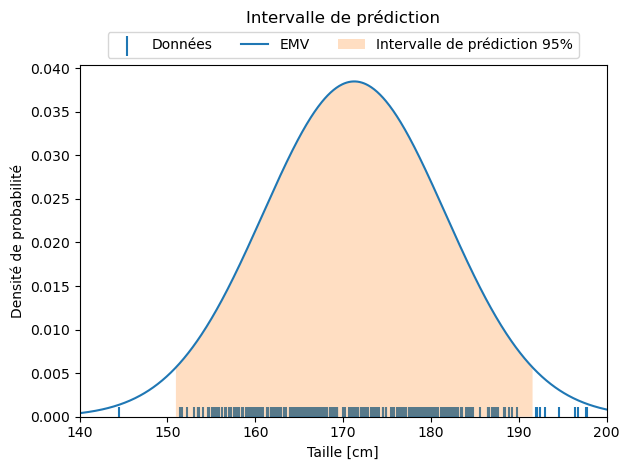
\includegraphics[width=1.0\linewidth]{Images/intervalle_prediction_n300}
				\label{fig:intervalle-prediction-n300}
			\end{figure}
		\end{column}
		\begin{column}{0.5\textwidth}
			\begin{figure}
				\centering
				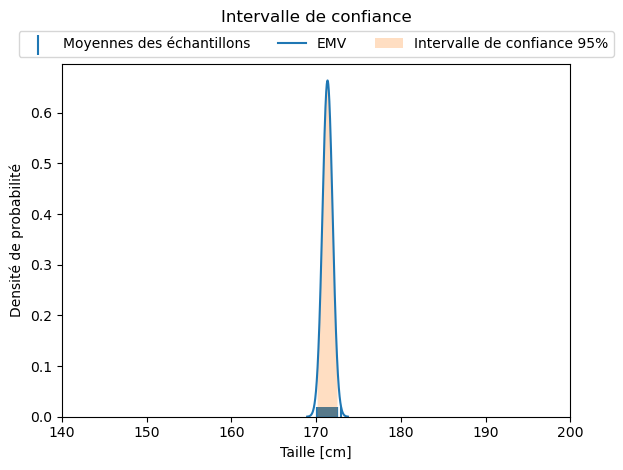
\includegraphics[width=1.0\linewidth]{Images/intervalle_confiance_n300}
				\label{fig:intervalle-confiance-n300}
			\end{figure}
		\end{column}
	\end{columns}
\end{frame}

\begin{frame}{Discussion}
	\begin{itemize}
		\item L'intervalle de prédiction ne change que très légèrement en augmentant la taille de l'échantillon.
		\item L'intervalle de confiance se resserre en augmentant la taille d'échantillon.
		\item L'intervalle de prédiction mesure la disparité de taille au sein d'un échantillon.
		\item L'intervalle de confiance mesure la disparité de la moyenne de plusieurs échantillons.
	\end{itemize}
	\pause
	\vspace{0.5cm}
	L'écart type de l'intervalle de confiance, appelé \textbf{erreur type} ($\ET$), se réduit quand la taille de l'échantillon augmente. Il varie en $1 / \sqrt{n}$.
\end{frame}

\begin{frame}{Interprétation}
	\begin{itemize}
		\item Un intervalle de prédiction à 95\% signifie que 95\% des futures observations se situeront dans cet intervalle.
		\pause
		\item Un intervalle de confiance à 95\% signifie que 95\% des futures moyennes d'échantillons, calculées d'une manière identique, se situeront dans cet intervalle.
		\pause
		\item Attention, la couverture de 95\% n'est pas \textbf{garantie}. Elle dépend de la validité des hypothèses, notamment de la nature Gaussienne des distributions.
	\end{itemize}
	\pause
	Si l'écart type de la taille d'un groupe d'étudiants $\sigma$ est connue, l'erreur type $\ET$ peut se calculer à partir de la taille d'échantillon $n$:
	\begin{equation}
		\ET = \frac{\sigma}{\sqrt{n}}
		\nonumber
	\end{equation}
\end{frame}

\subsection[Définitions]{Définitions}

\begin{frame}{Application à l'apprentissage automatique}
	\begin{itemize}
		\item Dans l'exemple précédent, nous nous sommes intéressés à une variable aléatoire $Y$ (taille des étudiants) et à un paramètre $\theta$ associé à cette variable aléatoire: la taille moyenne.
		\pause
		\item Dans le cas général de l'apprentissage automatique, nous nous intéresserons à une loi conditionnelle $Y \mid X$. L'objectif étant d'obtenir un modèle $\hat{f}$ de l'espérance conditionnelle $\E{Y \mid X}$.
	\end{itemize}
\end{frame}

\begin{frame}{Région de prédiction}
	\begin{block}{Définition: Région de prédiction}
		Soit un échantillon d'apprentissage $\mathcal{D} = \{\left(x^{(1)}, y^{(1)}\right), \cdots, \left(x^{(n)}, y^{(n)}\right)\}$ et une nouvelle observation $\left(x^{(n+1)}, y^{(n+1)}\right)$ issue de la même distribution. Une \textbf{région de prédiction} de niveau $1 - \alpha$ est une fonction $C$ qui, pour toute valeur $x^{(n+1)}$ produit un ensemble $C(x^{(n+1)})$ tel que:
		\begin{equation}
			P\left(y^{(n+1)} \in C\left(x^{(n+1)}\right)\right) \ge 1 - \alpha
			\nonumber
		\end{equation}
		Si $Y$ est une variable aléatoire continue (régression), alors $C$ est un \textbf{intervalle}. Si $Y$ est une variable aléatoire discrète (classification) alors $C$ est un \textbf{ensemble} de classes. 
	\end{block}
\end{frame}

\begin{frame}{Intervalle de confiance}
	\begin{block}{Définition: Intervalle de confiance}
		Un intervalle de confiance de niveau $1 - \alpha$ pour la fonction vraie $f$ est un intervalle $\left[L(x), U(x)\right]$ tel que:
		\begin{equation}
			P\left(L(x) \le f(x) \le U(x)\right) \ge 1 - \alpha
			\nonumber
		\end{equation}
		Si $Y$ est une variable aléatoire continue (régression), $f(x): \mathcal{X} \to \mathcal{Y}$ représente l'\textbf{espérance conditionnelle} $\E{Y \mid X}$. Si $Y$ est une variable aléatoire discrète, $f(x): \mathcal{X} \to ]0, 1[$ représente la \textbf{probabilité} d'appartenir à une classe $K$: $P(Y = K \mid X)$.
	\end{block}
\end{frame}

%=======================================================================================

\section[Modèles linéaires]{Modèles linéaires}

\begin{frame}{Approche théorique}
	Les modèles linéaires disposent d'un cadre \textbf{théorique} permettant de dériver ces intervalles ou ensembles. C'est ce que nous couvrirons dans cette section.
\end{frame}

\subsection[Régression linéaire]{Régression linéaire}

\begin{frame}{Hypothèses pour la régression linéaire}
	Pour la régression linéaire, les hypothèses déjà considérées sont encore d'actualité et même encore plus pertinentes:
	\begin{itemize}
		\item \textbf{Exogénéité}: $\E{\epsilon \mid X} = 0$
		\item \textbf{Homoscédasticité}: $\Var{\epsilon \mid X} = \sigeps$
		\item \textbf{Indépendance}: $\Cov{\epsilon^{(i)}, \epsilon^{(j)}} = 0 \quad \forall i \ne j$
	\end{itemize}
	Ces hypothèses sont appelées hypothèses de \textbf{Gauss-Markov}.
\end{frame}

\begin{frame}{Covariance de $\hat{\beta}$}
	Dans le cadre des hypothèses de Gauss-Markov (exogénéité, homoscédasticité et indépendance), la théorie de la régression des moindres carrés ordinaires, pour une application d'augmentation $\Phi: \mathcal{X} \to \tilde{\mathcal{X}}$, conduit à la matrice de covariance suivante pour $\hat{\beta}$ dans $\mathcal{M}_{d+1, d+1}\left(\mathbb{R}\right)$:
	\begin{equation}
		\Cov{\hat{\beta}} = \sigeps \left(\Phi(X)^T \Phi(X)\right)^{-1}
		\nonumber
	\end{equation}
	\pause
	En général, $\sigeps$ est inconnu. Il peut être estimé à partir de la variance des résidus $r = y - \hat{y}$:
	\begin{equation}
		s^2 = \frac{\text{SS}_{\text{res}}}{n - p} = \frac{\sum_{i=1}^n \left(y^{(i)} - \hat{y}^{(i)}\right)^2}{n - p}
		\nonumber
	\end{equation}
	Où $n$ est le nombre d'observations et $p = d + 1$ est le nombre de paramètres du modèle. $n - p$ est le nombre de degrés de liberté des résidus. Diviser par cette quantité permet d'obtenir un estimateur de variance $s^2$ non biaisé.
\end{frame}

\begin{frame}{Variance de $\hat{\beta}$}
	On peut déduire de la matrice de covariance la variance de $\hat{\beta}$ $\Var{\hat{\beta}} \in \mathcal{M}_{d+1, 1}\left(\mathbb{R^+}\right)$ en prenant les termes diagonaux de $\Cov{\hat{\beta}}$:
	\begin{equation}
		\Var{\hat{\beta}} = \diag \left(\Cov{\hat{\beta}}\right)
		\nonumber
	\end{equation}
	\pause
	L'écart type $\ET[\hat{\beta}] \in \mathcal{M}_{d+1, 1}\left(\mathbb{R+}\right)$ peut alors se déduire facilement:
	\begin{equation}
		\ET[\hat{\beta}] = \sqrt{\Var{\hat{\beta}}}
		\nonumber
	\end{equation}
\end{frame}

\begin{frame}{Connexion à l'estimation mono-dimensionnelle}
	Dans la section précédente, nous avons vu que nous pouvions estimer l'erreur type à partir de l'écart type d'une observation:
	\begin{equation}
		\ET = \frac{\sigma}{\sqrt{n}}
		\nonumber
	\end{equation}
	Dans le modèle de régression linéaire, si nous prenons l'application d'augmentation $\Phi: x \mapsto 1$ alors $\beta$ est maintenant un scalaire:
	\begin{equation}
		\begin{aligned}
			\Var{\hat{\beta}} &= \sigeps \left(\Phi(X)^T \Phi(X)\right)^{-1} \\
			                  &= \sigeps \left(\begin{pmatrix}
			                  	1 & 1 & \cdots & 1
			                  \end{pmatrix}\begin{pmatrix}
			                  1 \\ 1 \\ \vdots \\ 1
			                  \end{pmatrix}
			                  \right)^{-1} \\
			                  &= \sigeps \left(n\right)^{-1}
		\end{aligned}
		\nonumber
	\end{equation}
	Ce qui conduit à une erreur type semblable à celle vue auparavant $ET = \frac{\sigma_{\epsilon}}{\sqrt{n}}$	
\end{frame}

\begin{frame}{Variance de $\hat{Y}$}
	La variance de $\hat{Y} \mid X$, notée $\Var{\hat{Y} \mid X} \in \mathcal{M}_{n,1}(\mathbb{R})$ peut alors se calculer comme suit:
	\begin{equation}
		\Var{\hat{Y} \mid X} = \diag \left(\Phi(X) \Cov{\hat{\beta}} \Phi(X)^T\right)
		\nonumber
	\end{equation}
	\pause
	Et par conséquent, on a l'erreur type suivante:
	\begin{equation}
		\ET[\hat{Y} \mid X] = \sqrt{\Var{\hat{Y} \mid X}}
		\nonumber
	\end{equation}	
	\pause
	En supposant que les $\epsilon^{(i)}$ suivent une loi normale $\mathcal{N}(0, \sigeps)$ on peut alors déterminer un intervalle de confiance, soit sur $\hat{\beta}$, soit sur $\hat{Y}$.
\end{frame}

\begin{frame}{Intervalles de confiance}
	Notons $\varphi$ la fonction de densité de probabilité cumulée d'une loi normale standard $\mathcal{N}(0, 1)$. L'intervalle de confiance d'un niveau $1-\alpha$, noté $\text{IC}_{1-\alpha}$ pour $\hat{\beta}$ est donc:
	\begin{equation}
		\text{IC}_{1-\alpha}\left(\hat{\beta}\right) = \left[\hat{\beta} \pm \varphi^{-1}(1-\alpha / 2) \sqrt{\Var{\hat{\beta}}}\right]
		\nonumber
	\end{equation}
	\pause
	Pour la prédiction $\hat{Y} \mid X$, l'intervalle de confiance d'un niveau $1-\alpha$ est:
	\begin{equation}
		\begin{split}
			\text{IC}_{1-\alpha}\left(\hat{Y} \mid X\right) = \Biggl[ \hat{Y} \pm \varphi^{-1}(1-\alpha / 2) \sqrt{\Var{\hat{Y} \mid X}} \Biggr]
		\end{split}
		\nonumber
	\end{equation}
	\pause
	Note: Comme $\sigeps$ est généralement inconnue, il est classique d'utiliser une loi de Student avec $n - p$ degrés de liberté $\mathcal{T}(n - p)$ à la place de la loi normale standard.
\end{frame}

\begin{frame}{Intervalle de prédiction}
	L'intervalle de prédiction d'un niveau $1-\alpha$, noté $\text{IP}_{1-\alpha}$, pour la prédiction $\hat{Y} \mid X$ est:
	\begin{equation}
		\begin{split}
			\text{IP}_{1-\alpha}\left(\hat{Y} \mid X\right) = \Biggl[ \hat{Y} \pm \varphi^{-1}(1-\alpha / 2) \sqrt{\sigeps + \Var{\hat{Y} \mid X}} \Biggr]
		\end{split}
		\nonumber
	\end{equation}
	\pause
	Noter qu'il suffit d'ajouter $\sigeps$ à la variance de $\hat{Y} \mid X$ pour passer de l'intervalle de confiance à l'intervalle de prédiction.
\end{frame}

\subsection[Régression logistique]{Régression logistique}

\begin{frame}{Définitions supplémentaires}
	Nous aurons besoin de quelques définitions complémentaires associées à des problèmes de classification.
	\begin{block}{Définition: cote}
		La \textbf{cote} est un nombre réel dans $[0, +\infty[$ qui représente le rapport entre une probabilité d'un événement et la probabilité complémentaire de ce même événement:
		\begin{equation}
			\cote = \frac{p}{1 - p}
			\nonumber
		\end{equation}
	\end{block}
	\pause
	\begin{itemize}
		\item Si $p=0.5$, la cote est de $1$ (une chance sur deux).
		\item Si $p=0.8$, la cote est de $4$ (quatre contre un).
	\end{itemize}	
\end{frame}

\begin{frame}{Définitions supplémentaires}
	\begin{block}{Définition: logit}
		Le \textbf{logit} est un nombre réel dans $]-\infty, +\infty[$ qui représente le logarithme d'une cote:
		\begin{equation}
			\logit{p} = \ln{\left(\frac{p}{1 - p}\right)}
			\nonumber
		\end{equation}
	\end{block}
	\pause
	\begin{itemize}
		\item Si $p=0.5$, la cote est de $1$ et le logit est de $0$.
		\item Si $p=0.8$, la cote est de $4$ et le logit est approximativement $1.387$.
	\end{itemize}	
\end{frame}

\begin{frame}{Définitions supplémentaires}
	\begin{block}{Définition: score prédit}
		Dans un problème de régression logistique, on définit le \textbf{score}, un nombre réel dans $]-\infty, +\infty[$, comme la prédiction réalisée par le modèle linéaire:
		\begin{equation}
			\score{x} = \Phi(x) \hat{\beta}
			\nonumber
		\end{equation}
	\end{block}
\end{frame}

\begin{frame}{Définitions supplémentaires}
	\begin{block}{Définition: probabilité prédite}
		Dans un problème de régression logistique, on définit la \textbf{probabilité}, notée $\hat{p} \in ]0, 1[$, comme la prédiction réalisée par le modèle linéaire transformée par la fonction logistique $\sigma$:
		\begin{equation}
			\hat{p}(x) = \sigma\left(\score{x}\right) = \sigma\left(\Phi(x) \hat{\beta}\right)
			\nonumber
		\end{equation}
	\end{block}
\end{frame}

\begin{frame}{Dérivation}
	Calculer le logit de la probabilité prédite revient à effectuer le calcul suivant:
	\begin{equation}
		\begin{aligned}
			\logit{\hat{p}(x)}
			&= \ln{\left(\frac{\hat{p}(x)}{1 - \hat{p}(x)}\right)}
			= \ln{\left(\frac{\sigma(\score{x})}{1 - \sigma(\score{x})}\right)} \\
			&= \ln{\left(\frac{1}{1 + \exp{(-\score{x})}} \frac{1}{1 - \frac{1}{1 + \exp{(-\score{x})}}}\right)} \\
			&= \ln{\left(\frac{1}{1 + \exp{(-\score{x})}} \frac{1}{\frac{\exp{(-\score{x})}}{1 + \exp{(-\score{x})}}}\right)} \\
			&= \ln{\left(\frac{1}{\exp{(-\score{x})}}\right)} = \score{x}
		\end{aligned}
		\nonumber
	\end{equation}
\end{frame}

\begin{frame}{Dérivation}
	Dans un problème de régression logistique, le score et le logit représentent la \textit{même} quantité. Cela traduit la nature linéaire de la régression logistique: c'est une régression linéaire sur le score, \textit{enrobée} dans une fonction logistique pour calculer des probabilités !
\end{frame}

\begin{frame}{Revisite de l'incertitude en régression linéaire}
	En régression linéaire, nous avons pris l'hypothèse que la variance $\sigeps$ est constante (c'est notre hypothèse d'homoscédasticité). Nous avons écrit que la matrice de covariance est:
	\begin{equation}
		\Cov{\hat{\beta}} = \sigeps \left(\Phi(X)^T \Phi(X)\right)^{-1}
		\nonumber
	\end{equation}
	En introduisant une matrice diagonale $W \in \mathcal{M}_{n,n}(\mathbb{R})$:
	\begin{equation}
		W = \frac{1}{\sigeps} I_n
		\nonumber
	\end{equation}
	On peut dériver une formulation équivalente de la covariance des estimations $\beta$:
	\begin{equation}
		\Cov{\hat{\beta}} = \sigeps \left(\Phi(X)^T \Phi(X)\right)^{-1} = \left(\Phi(X)^T W \Phi(X)\right)^{-1}
		\nonumber
	\end{equation}	
\end{frame}

\begin{frame}{Incertitude en régression logistique}
	\begin{itemize}
		\item Comme la régression logistique résout un problème de régression linéaire sur le logit (ou le score), il est naturel de définir une matrice de poids $W$ basée sur la variance du logit.
		\pause
		\item On rappelle que chaque observation est associée à une loi de Bernoulli. Mais comme chaque paramètre de la loi de Bernoulli est différent, on doit utiliser une variance différente pour chaque observation.
		\pause
		\item La variance d'une variable aléatoire $Y^{(i)}$ suivant une loi de Bernoulli de paramètre $p^{(i)}$ est donnée par $p^{(i)} \left(1 - p^{(i)}\right)$.
		\pause
		\item On pourrait montrer que la variance de $\logit{p^{(i)}}$ est alors: 
		\begin{equation}
			\Var{\logit{p^{(i)}}} = \frac{1}{p^{(i)}\left(1 - p^{(i)}\right)}
			\nonumber
		\end{equation}
	\end{itemize}
\end{frame}

\begin{frame}{Incertitude en régression logistique}
	On peut donc définir, pour la régression logistique, une nouvelle matrice de poids $W$ telle que:
	\begin{equation}
		W_{ij} = \begin{cases}
			0 & \text{si} \, i \ne j \\
			\hat{p}^{(i)}\left(1 - \hat{p}^{(i)}\right) & \text{sinon}
		\end{cases}
		\nonumber
	\end{equation}
	\pause
	Et on en déduit la matrice de covariance de $\hat{\beta}$ pour la régression logistique:
	\begin{equation}
		\Cov{\hat{\beta}} = \left(\Phi(X)^T W \Phi(X)\right)^{-1}
		\nonumber
	\end{equation}
	\pause
	Et la variance de $\hat{\beta}$:
	\begin{equation}
		\Var{\hat{\beta}} = \diag \left(\Cov{\hat{\beta}}\right)
		\nonumber
	\end{equation}	
\end{frame}

\begin{frame}{Intervalle de confiance sur $\hat{\beta}$}
	Comme il s'agit de la partie linéaire du modèle pour calculer le score, on peut faire la même hypothèse que pour le modèle de régression linéaire, c'est à dire supposer que les incertitudes sur le score sont de type Gaussien. L'intervalle de confiance au niveau $1 - \alpha$ sur $\hat{\beta}$ est alors:
	\begin{equation}
			\text{IC}_{1-\alpha}\left(\hat{\beta}\right) = \left[\hat{\beta} \pm \varphi^{-1}(1 - \alpha/2) \sqrt{\Var{\hat{\beta}}}\right]
		\nonumber
	\end{equation}	
\end{frame}

\begin{frame}{Intervalle de confiance sur le logit ou le score}
	Pour une nouvelle observation $x^{(n+1)}$, on obtient d'abord la variance sur le score linéaire (le logit):
	\begin{equation}
		\Var{\logit{\hat{p}\left(x^{(n+1)}\right)}} = \diag\left(\Phi(x^{(n+1)}) \Cov{\hat{\beta}} \Phi(x^{(n+1)})^T\right)
		\nonumber
	\end{equation}
	\pause
	Puis, l'intervalle de confiance au niveau $1-\alpha$ sur le score (ou logit) se définit donc comme:
	\begin{equation}
		\begin{split}
			\text{IC}_{1-\alpha}\left(\logit{\hat{p}\left(x^{(n+1)}\right)}\right) = \bigg[
			&\logit{\hat{p}\left(x^{(n+1)}\right)} \\
			&\pm \varphi^{-1}(1 - \alpha/2) \sqrt{\Var{\logit{\hat{p}\left(x^{(n+1)}\right)}}}\bigg]			
		\end{split}
		\nonumber
	\end{equation}
\end{frame}

\begin{frame}{Intervalle de confiance sur la probabilité}
	En appliquant la fonction logistique $\sigma$ à l'intervalle précédent on obtient l'intervalle de confiance au niveau $1 - \alpha$ de la probabilité $\hat{p}(x^{(n+1)})$:
	\begin{equation}
		\begin{aligned}
			&\hat{p}_{\text{inf}} = \sigma\left(\logit{\hat{p}\left(x^{(n+1)}\right)} - \varphi^{-1}(1 - \alpha/2) \sqrt{\Var{\logit{\hat{p}\left(x^{(n+1)}\right)}}}\right) \\
			&\hat{p}_{\text{sup}} = \sigma\left(\logit{\hat{p}\left(x^{(n+1)}\right)} + \varphi^{-1}(1 - \alpha/2) \sqrt{\Var{\logit{\hat{p}\left(x^{(n+1)}\right)}}}\right) \\
			&\text{IC}_{1-\alpha}\left(\hat{p}\left(x^{(n+1)}\right)\right) = \left[\hat{p}_{\text{inf}}, \hat{p}_{\text{sup}}\right]
		\end{aligned}
		\nonumber
	\end{equation}
\end{frame}

\begin{frame}{Espace de prédiction sur la classe}
	Dans un problème de classification binaire, $\hat{p}\left(x^{(n+1)}\right)$ représente en fait $P(y^{(n+1)} = 1 \mid x^{(n+1)})$. \\
	En fonction de la valeur de $\hat{p}_{\text{inf}}$ et de $\hat{p}_{\text{sup}}$ on peut alors définir l'espace de prédiction au niveau $1 - \alpha$ comme suit:
	\begin{equation}
		C\left(x^{(n+1)}\right) = 
		\begin{cases}
			\{0\} & \text{si} \, \hat{p}_{\text{sup}} \le \alpha \\
			\{1\} & \text{si} \, \hat{p}_{\text{inf}} \ge 1 - \alpha \\
			\{0, 1\} & \text{sinon}
		\end{cases}
		\nonumber
	\end{equation}
	\pause
	\begin{itemize}
		\item Si $\text{IC}_{95\%}\left(\hat{p}\left(x^{(n+1)}\right)\right) = [0.92, 0.98]$ alors $C\left(x^{(n+1)}\right) = \{0, 1\}$.
		\item Si $\text{IC}_{95\%}\left(\hat{p}\left(x^{(n+1)}\right)\right) = [0.01, 0.03]$ alors $C\left(x^{(n+1)}\right) = \{0\}$.
		\item Si $\text{IC}_{95\%}\left(\hat{p}\left(x^{(n+1)}\right)\right) = [0.98, 0.99]$ alors $C\left(x^{(n+1)}\right) = \{1\}$.
	\end{itemize}
\end{frame}

%=======================================================================================

\section[Détermination empirique]{Détermination empirique}

\begin{frame}{Détermination empirique}
	\begin{itemize}
		\item Les régressions linéaire et logistique sont des algorithmes simples mais avec une théorie solide pour dériver des intervalles de confiances et des régions de prédictions à partir d'\textbf{un seul apprentissage}.
		\pause
		\item Ce n'est malheureusement pas le cas de tous les algorithmes d'apprentissage que l'on étudiera dans ce cours.
		\pause
		\item Dans cette section on verra comment on peut obtenir ces intervalles et régions de manière \textbf{empirique} et on comparera les résultats empiriques et théoriques obtenus précédemment.
		\item On utilisera l'algorithme du \textbf{bootstrapping} pour générer de \textbf{multiples} apprentissages et ainsi dériver ces intervalles et régions.
	\end{itemize}
\end{frame}

\begin{frame}{Notations pour les algorithmes}
	\begin{itemize}
		\item On note les $n$ observations des données d'apprentissage $\mathcal{D} = \{(x^{(i)}, y^{(i)})\}_{i=1}^n$.
		\item On note $\mathcal{D}^{(b)} \text{  pour  } b=1, 2, \cdots B$ les $B$ bootstraps générés.
		\item On note ${X_i^{(1)}, X_i^{(2)}, \cdots, X_i^{(m)}}$ les $m$ caractéristiques d'entrée pour l'inférence.
		\item On note $a: \mathcal{M}_{n,1}(\mathbb{R}) \to \mathbb{R}$ une fonction qui retourne un élément aléatoire d'un vecteur colonne $A$ en suivant une loi uniforme: $a(A) = A_j, \, j \sim \mathcal{U}(1, 2, \cdots, n)$.
	\end{itemize}
\end{frame}

\begin{frame}[allowframebreaks]{Régression linéaire}
	\begin{enumerate}
		\item Calculer $\hat{\beta}$ en utilisant toutes les données d'apprentissage $\mathcal{D}$ avec la méthode des moindres carrés.
		\item Calculer les résidus sur $\mathcal{D}$: $R = Y - \hat{Y}$.
		\item Répéter les étapes suivantes pour chaque bootstrap $b$:
			\begin{itemize}
				\item Déterminer les données d'apprentissage $\mathcal{D}^{(b)}$.
				\item Calculer $\hat{\beta}^{(b)}$ par la méthode des moindres carrés sur $\mathcal{D}^{(b)}$.
				\item Calculer $\hat{Y}_i^{(b)}$ à partir des données d'inférence $X_i$: $\hat{Y}_i^{(b)} = \Phi(X_i) \hat{\beta}^{(b)}$.
			\end{itemize}
		\item Pour chaque entrée $k$ de $X_i$, calculer les quantiles $\alpha / 2$ et $1 - \alpha / 2$ sur $\{\left(\hat{y}_i^{(k)}\right)^{(1)}, \left(\hat{y}_i^{(k)}\right)^{(2)}, \cdots, \left(\hat{y}_i^{(k)}\right)^{(B)}\}$. Cela donne l'intervalle de confiance au niveau $1 - \alpha$ pour $X_i^{(k)}$.
		\item Pour chaque entrée $k$ de $X_i$ et pour chaque bootstrap $b$, associer aléatoirement un résidu aux prédictions: $\left(\hat{y}_i^{*(k)}\right)^{(b)} = \left(\hat{y}_i^{(k)}\right)^{(b)} + a(R)$.
		\item Pour chaque entrée $k$ de $X_i$, calculer les quantiles $\alpha / 2$ et $1 - \alpha / 2$ sur $\{\left(\hat{y}_i^{*(k)}\right)^{(1)}, \left(\hat{y}_i^{*(k)}\right)^{(2)}, \cdots, \left(\hat{y}_i^{*(k)}\right)^{(B)}\}$. Cela donne l'intervalle de prédiction au niveau $1 - \alpha$ pour $X_i^{(k)}$.
	\end{enumerate}
\end{frame}

\begin{frame}{Exemple: régression linéaire}
	\begin{columns}
		\begin{column}{0.5\textwidth}
			\begin{figure}
				\centering
				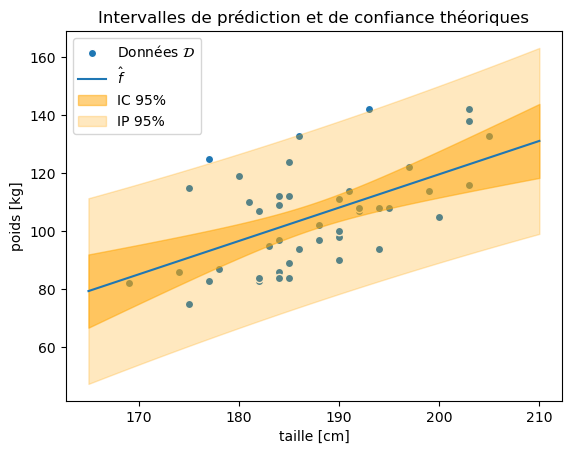
\includegraphics[width=1.0\linewidth]{Images/IP_IC_lineaire_theorie}
				\label{fig:IP_IC_lineaire_theorie}
			\end{figure}
		\end{column}
		\begin{column}{0.5\textwidth}
			\begin{figure}
				\centering
				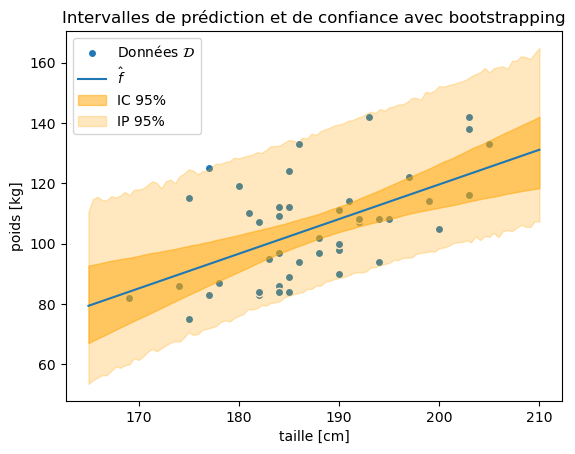
\includegraphics[width=1.0\linewidth]{Images/IP_IC_lineaire_bootstrap}
				\label{fig:IP_IC_lineaire_bootstrap}
			\end{figure}
		\end{column}
	\end{columns}
	Nous obtenons des résultats très similaires avec la théorie et avec un bootstrapping.
\end{frame}

\begin{frame}[allowframebreaks]{Régression logistique}
	\begin{enumerate}
		\item Calculer $\hat{\beta}$ en utilisant toutes les données d'apprentissage $\mathcal{D}$ avec la méthode des moindres carrés.
		\item Répéter les étapes suivantes pour chaque bootstrap $b$:
		\begin{itemize}
			\item Déterminer les données d'apprentissage $\mathcal{D}^{(b)}$.
			\item Calculer $\hat{\beta}^{(b)}$ par la méthode des moindres carrés sur $\mathcal{D}^{(b)}$.
			\item Calculer $\hat{p}_i^{(b)}$ à partir des données d'inférence $X_i$: $\hat{p}_i^{(b)} = \sigma\left(\Phi(X_i) \hat{\beta}^{(b)}\right)$.
		\end{itemize}
		\item Pour chaque entrée $k$ de $X_i$, calculer les quantiles $\alpha / 2$ et $1 - (\alpha / 2)$ sur $\{\left(\hat{p}_i^{(k)}\right)^{(1)}, \left(\hat{p}_i^{(k)}\right)^{(2)}, \cdots, \left(\hat{p}_i^{(k)}\right)^{(B)}\}$. Cela donne l'intervalle de confiance au niveau $1 - \alpha$ pour $X_i^{(k)}$.
		\item Pour chaque entrée $k$ de $X_i$, on détermine l'espace de prédiction $C\left(x_i^{(k)}\right)$ d'une manière similaire à l'approche théorique:
		\begin{equation}
			C\left(x_i^{(k)}\right) = 
			\begin{cases}
				\{0\} & \text{si} \, \hat{p}_{1-\alpha/2}^{(k)} \le \alpha \\
				\{1\} & \text{si} \, \hat{p}_{\alpha/2}^{(k)} \ge 1 - \alpha \\
				\{0, 1\} & \text{sinon}
			\end{cases}
			\nonumber
		\end{equation}		
	\end{enumerate}
\end{frame}

\begin{frame}{Exemple: régression logistique}
	\begin{columns}
		\begin{column}{0.5\textwidth}
			\begin{figure}
				\centering
				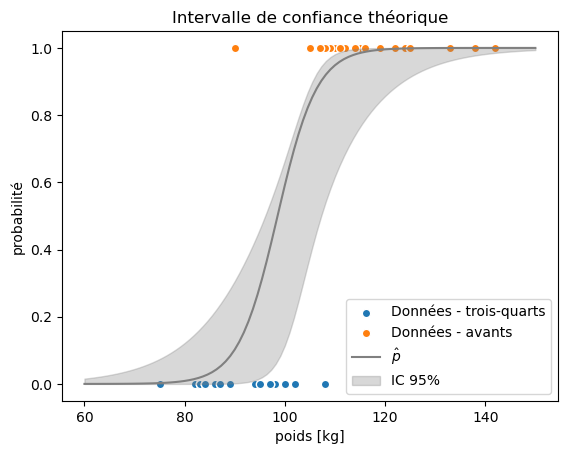
\includegraphics[width=1.0\linewidth]{Images/IP_IC_logistique_theorie}
				\label{fig:IP_IC_logistique_theorie}
			\end{figure}
		\end{column}
		\begin{column}{0.5\textwidth}
			\begin{figure}
				\centering
				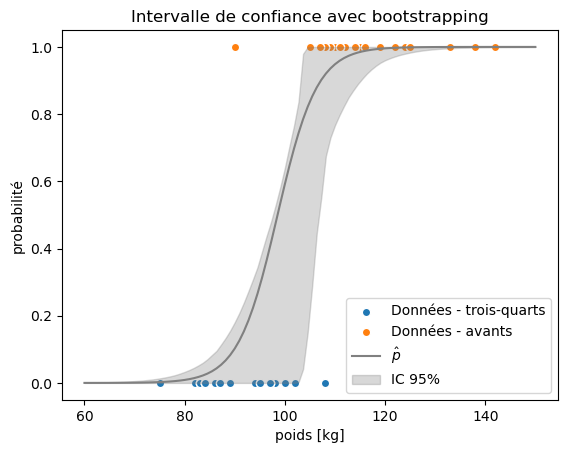
\includegraphics[width=1.0\linewidth]{Images/IP_IC_logistique_bootstrap}
				\label{fig:IP_IC_logistique_bootstrap}
			\end{figure}
		\end{column}
	\end{columns}
	Nous obtenons des résultats assez similaires avec la théorie et avec un bootstrapping.
\end{frame}

\begin{frame}{Exemple: régression logistique}
	\begin{columns}
		\begin{column}{0.5\textwidth}
			\begin{figure}
				\centering
				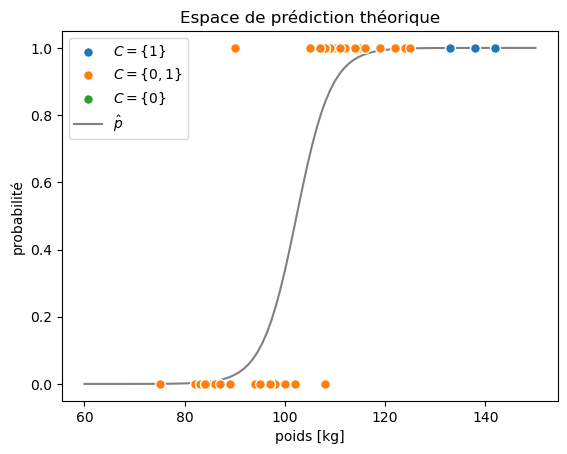
\includegraphics[width=0.95\linewidth]{Images/espace_prediction_theorique}
				\label{fig:espace_prediction_theorique}
			\end{figure}
		\end{column}
		\begin{column}{0.5\textwidth}
			\begin{figure}
				\centering
				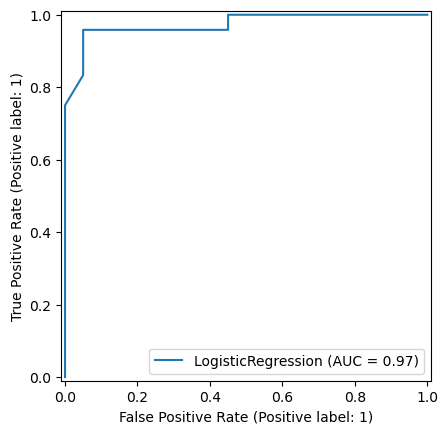
\includegraphics[width=0.85\linewidth]{Images/ROC}
				\label{fig:ROC}
			\end{figure}
		\end{column}
	\end{columns}
	Même si la courbe ROC montre que notre algorithme capture bien les tendances, l'espace de prédiction est beaucoup plus exigeant et ne montre que quelques (5) joueurs classés avec confiance comme des avants. Pour tous les autres joueurs, la régression logistique est beaucoup moins catégorique.
\end{frame}

\begin{frame}{Conclusions}
	\begin{itemize}
		\item Nous avons vu comment déterminer, par la théorie des régressions linéaire et logistique, les intervalles de confiance et les régions de prédiction.
		\pause
		\item Nous avons montré que pour les régressions linéaire et logistique, le cœur du calcul des intervalles et des régions est la matrice de covariance de $\hat{\beta}$ qui est déterminée à partir de toutes les données d'apprentissage. Elle est utilisée quelles que soient les entrées $X_i$ fournies ensuite au modèle.
		\pause
		\item Nous avons aussi estimé ces mêmes intervalles et régions en utilisant un algorithme de bootstrapping.
		\pause
		\item Nous avons vu que l'on obtient une bonne adéquation entre la théorie et la méthode du bootstrapping.
		\pause
		\item Nous avons aussi vu que la région de prédiction est une métrique bien plus contraignante que ne peut l'être la courbe ROC pour la classification.
	\end{itemize}
\end{frame}

\begin{frame}{Conclusions}
	\begin{itemize}
		\item Même si l'algorithme de bootstrapping a été utilisé pour les régressions linéaire et logistique, cet algorithme reste applicable \textbf{à tout} modèle de régression et de classification.
		\pause
		\item Pour une majorité de modèles, nous ne disposons pas d'éléments théoriques pour déterminer ces intervalles et espaces et les méthodes empiriques sont les seules disponibles. Mais elles nécessitent d'entrainer plusieurs modèles, ce qui peut se révéler \textbf{coûteux}.
		\pause
		\item L'intervalle de confiance fournit une estimation de la \textbf{variance} du modèle.
		\pause
		\item La région de prédiction englobe l'\textbf{ensemble des erreurs} (Bayes, erreur d'approximation ou biais, erreur d'estimation ou variance) mais ne permet pas de discriminer l'erreur d'approximation de l'erreur de Bayes.
	\end{itemize}
\end{frame}

\begin{frame}{Conclusions}
	\begin{itemize}
		\item Les régions de prédictions sont des outils \textbf{majeurs} de la validation de modèles d'apprentissage automatique utilisés dans des systèmes \textbf{critiques} pour la sécurité.
		\pause
		\item Des méthodes de \textbf{prédiction conforme} ont été développées plus récemment pour \textbf{garantir} statistiquement une couverture pour les régions de prédiction et s'appliquent à tous les modèles de régression et de classification.
	\end{itemize}
\end{frame}

\end{document}
